\documentclass{article}
\usepackage{graphicx} % Required for inserting images
\usepackage{amsmath}

\title{24.07.30 Schnorr MuSig and BLS Benchmark}
\author{Xun Zhang \quad \quad Wuyun Siqin \quad \quad Bingsheng Zhang \\ 
Zhejiang University, CHN \\
22221024@zju.edu.cn \quad 3210101763@zju.edu.cn \quad bingsheng@zju.edu.cn}

\date{July 30 2024}

\begin{document}

\maketitle

\section{Schnorr Multi-signature Scheme}

\subsection{Roadmap}

We give a roadmap to the existing Schnorr Multi-signature scheme(it's called 'MuSig' specifically).

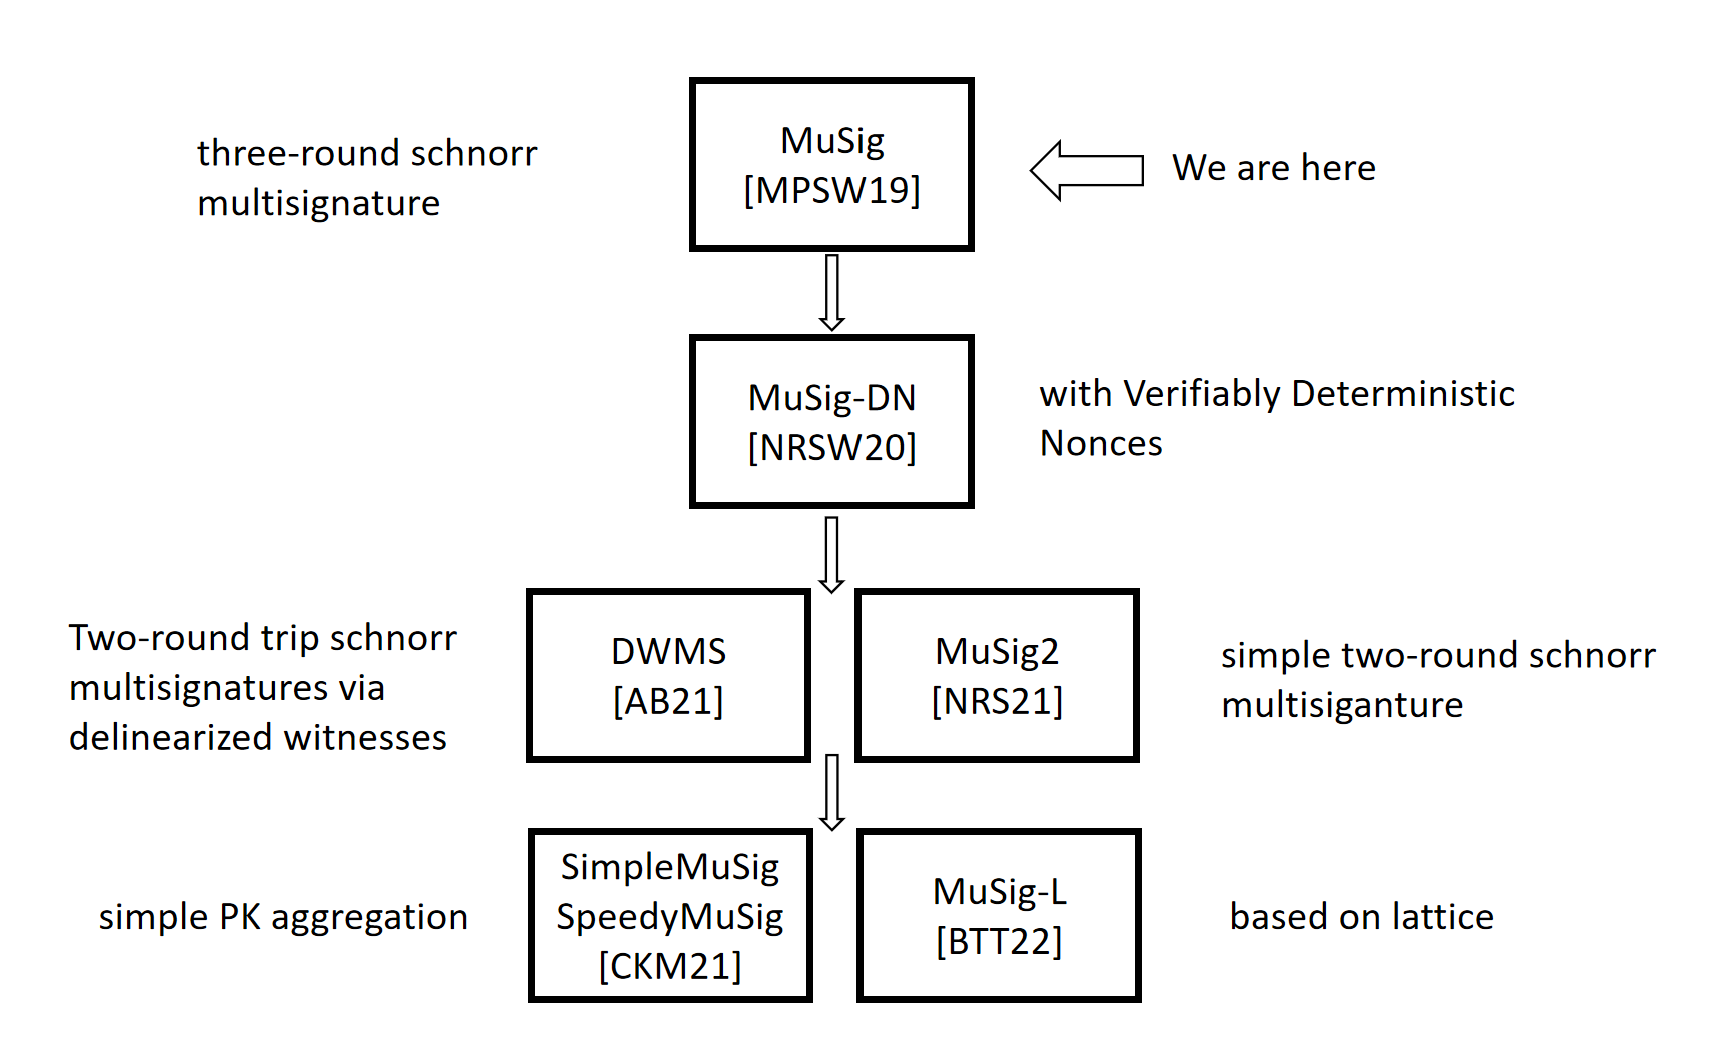
\includegraphics[width=1\linewidth]{roadmap.png}

The Schnorr multisignature we implemented is the paper [MPSW19], the scheme is called \textit{MuSig}. It is a three-round pratical schnorr multisignature with public key aggregation.

\subsection{MuSig [MPSW19]}

We try to give a detailed description to the MuSig scheme. Note that all the multisignature schemes involve all public keys to participate in signing.


\textbf{Round 1.}

A group of $n$ signers want to cosign a message $m$. Let 
$X_1$ and $x_1$ be the public and private key of a specific signer, let $X_1, ... , X_n$ be the public keys of other cosigners and let $\langle L \rangle$ be the multi-set of all public keys involved in the signing process.

For $i \in \{1,...,n\}$, the signer computes the following:

\[
a_i = \textrm{H}_{agg}(\langle L \rangle, X_i)
\]

as well as the “aggregated” public key:

\[
\tilde X = \prod_{i=1}^{n} X_i^{a_i}
\]


\textbf{Round 2.}

The signer generates a random private nonce $r_1$, computes $R_1 = g^{r_1}$ (the public nonce) and commitment $ t_{1} = \textrm{H}_{com}(R_{1}) $ and sends $t_{1}$ to all other cosigners.

When receiving the commitments $t_2,...,t_n$ from the other cosigners, the signer sends $R_1$ to all other cosigners. This ensures that the public nonce is not exposed until all commitments have been received.


Upon receiving $R_2,...,R_n$ from other cosigners, the signer verifies that $ t_{i} = \textrm{H}_{com}(R_{i}) $ for all $i \in \{2,...,n\}$.

The protocol is aborted if this is not the case.


\textbf{Round 3.}

If all commitment and random challenge pairs can be verified with $\textrm{H}_{agg}$, the following is computed:

\[
R = \prod_{i=1}^{n} R_i
\]
\[
c = \textrm{H}_{sig}(\tilde{X},R,m)
\]
\[
s_1 = r_1 + ca_1x_1
\]
Signature $s_1$ is sent to all other cosigners. When receiving $s_2,...,s_n$ from other cosigners, the signer can compute $s = \sum_{i=1}^{n}s_i \, \textrm{mod} \, p$. The signature is $\sigma=(R,s)$.

In order to verify the aggregated signature $\sigma=(R,s)$, given a lexicographically encoded multi-set of public keys $\langle L \rangle$and message $m$, the verifier computes:

\[
a_i = \textrm{H}_{agg}(\langle L \rangle, X_i)\quad \textrm{for} \quad i \in \{1,...,n\}
\]
\[
\tilde X = \prod_{i=1}^{n} X_i^{a_i}
\]
\[
c = \textrm{H}_{sig}(\tilde{X},R,m)
\]
then accepts the signature if:
\[
g^s = R \prod_{i=1}^{n}X_i^{a_ic} = R\tilde X^c
\]


\subsection{MuSig2 [NRS21]}

For the convenience of explanation, we just use a two-party setting.

\textbf{Round 1.}

This round is completely same as the original \textit{MuSig} scheme. But it can be more efficient by use a hash function:

\[
L = \textrm{H}(X_1 || X_2)
\]
\[
a_i = \textrm{H}_{agg}(L, X_i)
\]
\[
X = a_1X_1+a_2X_2
\]

\textbf{Round 2.}
The signer Alice generates \textbf{TWO} random private nonce $r_1'$ and $r_1''$, computes $R_1' = g^{r_1'}$ and $R_1'' = g^{r_1''}$(the public nonce), and sends them to Bob.

After receiving Bob's nonce $R_2'$ and $R_2''$, Alice do the follwing calculation:

\[
R' = R_1'+R_2'
\]
\[
R'' = R_1''+R_2''
\]

the coefficient used for nonce combination will be:
\[
b = \textrm{H}_{agg2}(X||R'||R''||m)
\]

and the final nonce as following:
\[
R_1 = R_1'+bR_1''
\]
\[
R_2 = R_2'+bR_2''
\]
\[
R = R_1+R_2
\]

the challenge will be:
\[
c = \textrm{H}_{sig}(\tilde{X},R,m)
\]
Now it's time for Alice to create her response $s1$ (Bob will create $s2$ in a similar fashion):
\[
r_1=r_1'+br_1''
\]
\[
s_1=r_1+ca_1x_1
\]

and the final multisignature is $(R,s) = (R, s_1+s_2)$

One can verify the signature just as a normal schnorr signature(after computing a aggregated public key $X$).

\subsection{SpeedyMuSig [CKM21]}

This work is from \textbf{Elizabeth Crites} et al. It construct a variant of the two-round multisignature scheme \textbf{MuSig2} that includes proofs of possession. And the public key aggregation is very simple(just multiply all the pks).

\textbf{Key Generation}.


Each signer will compute their own hash $\overline c = \textrm{H}_{reg}(X,X,\overline R)$. Where $\overline R$ is the commitment of random nonce $\overline R = g^{\overline r}$. Signer compute the signature $\overline z = \overline r +\overline c x$. Their proof of possession is the signature $\pi = (\overline R, \overline z)$.


\textbf{Key Verification.}


On input a public key $(X,\pi)$, the verifier computes $\overline c = \textrm{H}_{reg}(X,X,\overline R)$ and accepts if $\overline R X^{\overline c} = g^{\overline z}$.


\textbf{Round 1.}


Same as \textbf{MuSig2}, each signer generate their own $R'_i$ and $R''_i$.


\textbf{Round 2.}

Compute the simple aggregated public key:
\[
\tilde X = \prod_{i=1}^{n} X_i
\]

The other opration is totally same as \textbf{MuSig2}.

And the final signature is :
\[
s_i=r_i+cx_i
\]
This is a basic Schnorr signature. And the final multisignature is $(R,s) = (R, \sum s_i)$.

One can verify the signature just as \textbf{MuSig2}, but with a \textbf{simple} publick key aggregation.



\section{BLS Benchmark}


\subsection{Version 1: Built-in BLS Signatures in halo2-lib}
\subsubsection{Data Generation}
The data generation process for this version includes:
Randomly generating secret keys (\textit{sk}).
Deriving the public keys (\textit{pk}) and signatures (\textit{sig}) from the secret key.
Generating a random message hash (\textit{msg\_hash}).


\subsubsection{Code Description}

The BLS signature verification code is implemented in the \texttt{BlsSignatureChip} struct. The overview is as following.



\paragraph{Input Parameters} 

$G_1$:\{$g_1$, \text{pubkeys}\} , $G_2$ \{signatures, msghash\}.

\paragraph{Verification Process}
The function ensures that $e(g_1, \text{signature}) = e(\text{pubkey}, H(m))$ by verifying that $e(g_1, \text{signature}) \cdot e(\text{pubkey}, -H(m)) = 1$, where $e$ is the optimal Ate pairing.




\subsubsection{Benchmark Results}
The following table summarizes the benchmark results for different parameter settings, 

\textbf{Note:} For all benchmark results in Table \ref{tab:version1}, the \textit{Num Fixed} is 1, \textit{Num Limbs} is 3, and \textit{Num Aggregation} is 2.
\begin{table}[h]
    \centering
    \begin{tabular}{c|c|c|c|c|c|c|c} \hline
        Degree & Advice & Lookup & Lookup Bits & Limb Bits & Proof Time & Proof Size & Verify Time \\ \hline
        14 & 211 & 27 & 13 & 91 & 19.9237s & 95808 & 103.104ms \\ \hline
        15 & 105 & 14 & 14 & 90 & 17.3673s & 48000 & 78.1614ms \\ \hline
        16 & 50 & 6 & 15 & 90 & 16.3698s & 22752 & 70.8313ms \\ \hline
        17 & 25 & 3 & 16 & 88 & 16.6448s & 11520 & 72.8319ms \\ \hline
        18 & 13 & 2 & 17 & 88 & 18.9069s & 6080 & 82.6032ms \\ \hline
        19 & 6 & 1 & 18 & 90 & 19.2544s & 3072 & 85.9115ms \\ \hline
        20 & 3 & 1 & 19 & 88 & 26.3072s & 1920 & 96.7935ms \\ \hline
        21 & 2 & 1 & 20 & 88 & 40.4636s & 1344 & 131.228ms \\ \hline
        22 & 1 & 1 & 21 & 88 & 67.5031s & 960 & 203.219ms \\ \hline
    \end{tabular}
    \caption{Benchmark results for various degrees and parameters (Version 1)}
    \label{tab:version1}
\end{table}

\textbf{Note:} The configuration with Degree , Advice , Lookup , Fixed , Lookup Bits , Limb Bits , Num Limbs is 17, 25, 3, 1, 16, 88, and 3, respectively.

\begin{table}[h]
    \centering
    \begin{tabular}{c|c|c|c} \hline
        Num Aggregation & Proof Time & Proof Size & Verify Time \\ \hline
        2 & 17.4515s & 11520 & 72.7713ms \\ \hline
        200 & 22.3638s & 15008 & 89.0890ms \\ \hline
        2000 & 67.0237s & 45952 & 286.869ms \\ \hline
        4000 & 116.439s & 79680 & 327.100ms \\ \hline
        6000 & 165.035s & 113760 & 551.478ms \\ \hline
        8000 & 210.119s & 147840 & 664.927ms \\ \hline
        10000 & 256.993s & 181920 & 841.507ms \\ \hline
    \end{tabular}
    \caption{Benchmark results for varying aggregation sizes (Version 1)}
    \label{tab:version1_agg}
\end{table}


\subsection{Version 2: BLS with Merkle Tree and Hash of Message Verification}
\subsubsection{Data Generation}
The data generation process involves:
Generating a Merkle tree based on the specified depth \textit{d} with random sks and pks.
Recording the \textit{pk} and \textit{sk} values.

%Generating a random message of type \textit{F} and computing its hash.

Note: Data generation time increases linearly with depth; thus, data is pre-generated and read from JSON files.

\subsubsection{Code Description}

The combined BLS signature and Merkle tree verification code is implemented in the \texttt{CombineBlsMtChip} struct.  The overview is as following.

\paragraph{Input Parameters}
:

\textbf{g1}, \textbf{signatures}, \textbf{pubkeys} as the above.

\textbf{message}: An element of type \textit{F} representing the message.

\textbf{root}: The root of the Merkle tree.

\textbf{merkle\_infos}: Representing the Merkle tree information (leaf, path, and index).

\paragraph{Verification Process}
:
    
\textbf{BLS Signature Verification}: 
    As the above, where the hash of message is generated by the original message by calculate its poseidon hash.

\textbf{Merkle Tree Verification}:
    The function verifies the Merkle tree by comparing the computed hash from the leaf to the root of the Merkle tree for each path in the \textit{merkle\_infos}. 

\textbf{Combining Results}:
    The results from the BLS signature verification and the Merkle tree verification are combined using a logical AND operation. Additionally, the function ensures that the $x$ coordinate of each public key matches the corresponding Merkle tree leaf.



\subsubsection{Benchmark Results}
The following table summarizes the benchmark results for different parameter settings:

\textbf{Note:} The configuration with \textit{Degree, Advice, Lookup, Fixed, Lookup Bits, Limb Bits, Num Limbs} is fixed at 17, 25, 3, 1, 16, 88, and 3 respectively.

\begin{table}[h]
    \centering
    \begin{tabular}{c|c|c|c|c} \hline
        Num Aggregation & Num MT leaf & Proof Time & Proof Size & Verify Time \\ \hline
        16 & 32 & 20.5646s & 13152 & 80.7299ms \\ \hline
        32 & 64 & 21.1587s & 14528 & 74.7994ms \\ \hline
        64 & 128 & 26.8527s & 17984 & 106.079ms \\ \hline
        128 & 256 & 38.0101s & 25600 & 142.173ms \\ \hline
        256 & 512 & 62.4086s & 41632 & 223.739ms \\ \hline
        512 & 1024 & 110.867s & 76448 & 485.612ms \\ \hline
        1024 & 2048 & 217.888s & 150912 & 750.038ms \\ \hline
        2048 & 4096 & 456.445s & 310336 & 1.599s \\ \hline
    \end{tabular}
    \caption{Benchmark results for various aggregation sizes (Degree = 17)}
    \label{tab:degree17}
\end{table}

\textbf{Note:} The configuration with \textit{Degree, Advice, Lookup, Fixed, Lookup Bits, Limb Bits, Num Limbs} is fixed at 19, 6, 1, 1, 18, 90, and 3 respectively.

\begin{table}[h]
    \centering
    \begin{tabular}{c|c|c|c|c} \hline
        Num Aggregation & Num MT leaf & Proof Time & Proof Size & Verify Time \\ \hline
        16 & 32 & 21.2527s & 3424 & 93.9743ms \\ \hline
        32 & 64 & 23.7070s & 4000 & 99.2152ms \\ \hline
        64 & 128 & 26.5444s & 4576 & 123.859ms \\ \hline
        128 & 256 & 39.8745s & 7008 & 173.010ms \\ \hline
        256 & 512 & 59.3749s & 10688 & 248.074ms \\ \hline
        512 & 1024 & 102.120s & 19104 & 490.098ms \\ \hline
        1024 & 2048 & 199.642s & 37664 & 878.392ms \\ \hline
        2048 & 4096 & 415.307s & 77312 & 1.491s \\ \hline
    \end{tabular}
    \caption{Benchmark results for various aggregation sizes (Degree = 19)}
    \label{tab:degree19}
\end{table}

\textbf{Note:} The configuration with \textit{Degree, Advice, Lookup, Fixed, Lookup Bits, Limb Bits, Num Limbs} is fixed at 21, 2, 1, 1, 20, 88, and 3 respectively.

\begin{table}[h]
    \centering
    \begin{tabular}{c|c|c|c|c} \hline
        Num Aggregation & Num MT leaf & Proof Time & Proof Size & Verify Time \\ \hline
        16 & 32 & 45.8947s & 1696 & 196.018ms \\ \hline
        32 & 64 & 46.6231s & 1696 & 185.981ms \\ \hline
        64 & 128 & 50.6344s & 1920 & 202.661ms \\ \hline
        128 & 256 & 57.9435s & 2272 & 229.011ms \\ \hline
        256 & 512 & 79.8219s & 3424 & 356.260ms \\ \hline
        512 & 1024 & 118.136s & 5376 & 480.207ms \\ \hline
        1024 & 2048 & 208.207s & 9984 & 798.579ms \\ \hline
        2048 & 4096 & 416.241s & 19904 & 1.538s \\ \hline
    \end{tabular}
    \caption{Benchmark results for various aggregation sizes (Degree = 21)}
    \label{tab:degree21}
\end{table}

\subsubsection{Benchmark Environment}

\begin{tabular}{ll}
\textbf{OS} & Ubuntu 20.04.6 LTS (x86\_64) \\
\textbf{Kernel} & 5.4.0-169-generic \\
\textbf{CPU} & Intel Xeon Silver 4214 (48 cores) @ 3.200GHz \\
\textbf{GPU} & 4 x NVIDIA GeForce RTX 2080 Ti \\
\textbf{Memory} & 128546 MiB \\
\end{tabular}

\end{document}
